\documentclass[conference]{IEEEtran}
\usepackage[T1]{fontenc}
\usepackage{booktabs}
\usepackage{graphicx}
\usepackage{array}
\usepackage{url}
\usepackage{balance}
\setlength{\textfloatsep}{8pt plus 1pt minus 1pt}
\setlength{\floatsep}{8pt plus 1pt minus 1pt}
\setlength{\intextsep}{8pt plus 1pt minus 1pt}

\title{EdgePII: Lightweight Context-Aware PII Detection for Local Inference}
\author{
\IEEEauthorblockN{Vasishta Nandipati, Karthikeya Davasam, and Tirth Koradia}
\IEEEauthorblockA{Manipal Institute of Technology\\Manipal, India}
}

\begin{document}
\maketitle

\begin{abstract}
Text sent to a remote language model may contain personal information that is unrelated to the user's request. This paper studies whether compact encoder models can detect that information and estimate its relevance before any text leaves the device. EdgePII separates the problem into token-level detection and entity-level relevance classification. We compare MiniLM-L6-H384, DistilBERT-base-uncased, and BERT-base-uncased under common preprocessing, training, evaluation, and CPU measurement procedures. Three-seed CAPID pilots obtain strict typed span F1 of $0.504\pm0.039$, $0.729\pm0.024$, and $0.771\pm0.003$, respectively. Relevance macro-F1 is $0.705\pm0.018$, $0.738\pm0.008$, and $0.628\pm0.193$; the BERT result includes one retained majority-class collapse. A reduced AI4Privacy study shows that increasing usable training data from 4,930 to 9,854 documents improves every detector by 0.016--0.018 F1. At 10K, DistilBERT reaches 0.957 F1, compared with 0.959 for BERT, while requiring about half the median detector latency. Complete context-aware pipelines measure 345, 734, and 1,424 ms median on the study laptop. The prespecified 5\% irrelevant-character leakage criterion is infeasible for every model and seed because detector misses leak information even when all detected spans are masked. No tested architecture satisfies every deployment criterion. DistilBERT provides the strongest observed accuracy and efficiency compromise, but it does not provide a privacy guarantee.
\end{abstract}

\begin{IEEEkeywords}
PII detection, local inference, contextual relevance, lightweight transformers, privacy filtering
\end{IEEEkeywords}

\section{Introduction}
Applications built around remote language models often combine a user's question with notes, records, or conversation history. Some details in that context may support the task, while others create avoidable disclosure. A local filter can reduce exposure before transmission, but the filter must solve two different problems. It must first find personal information and then decide whether the requested task depends on that information.

Blanket masking is conservative, yet it can remove details required for a useful response. Context-aware retention preserves selected entities, but a relevance prediction cannot establish consent or authorization. A missed detector span also bypasses every later policy. These dependencies make end-to-end evaluation necessary.

CAPID studies contextual personally identifiable information (PII) detection with locally owned generative models~\cite{capid}. PII-Bench studies query-aware privacy protection across a broader benchmark~\cite{piibench}. Their findings motivate this work, but their protocols and model sizes differ from ours. EdgePII instead evaluates compact encoders that fit on a laptop CPU.

We address two research questions:
\begin{itemize}
    \item \textbf{RQ1:} What is the smallest tested transformer that maintains useful detection and relevance performance under declared memory, latency, and leakage constraints?
    \item \textbf{RQ2:} How does additional PII training data affect detection quality and computational cost?
\end{itemize}

The project makes four contributions. First, it implements an offset-preserving pipeline that harmonizes AI4Privacy and CAPID into a common 20-category representation. Second, it compares three encoders through one training and evaluation path, including sliding-window inference. Third, it evaluates detection, relevance, privacy leakage, latency, memory, question dependence, and domain shift. Finally, it provides pinned manifests, deterministic seeds, exclusion records, machine-readable results, and a local demonstration.

\section{Related Work}
CAPID frames privacy filtering as joint span, type, and question-relevance prediction. Its fine-tuned 3B model reports test span F1 of 0.9608 and relevance accuracy of 0.9306~\cite{capid}. Those values use a hybrid span metric on 200 samples, with type and relevance evaluated on matched spans. EdgePII uses strict exact typed character spans on a retained flat-span subset and evaluates relevance on gold spans. Direct numerical ranking would therefore be invalid.

PII-Bench v2 describes 2,842 samples with seven broad and 55 fine-grained categories~\cite{piibench}. It reports that relevance remains difficult for large prompted models. We verified published values from the paper, but we did not obtain or reproduce its dataset. PII-Bench values appear only as related-work references.

AI4Privacy PII-200K supplies larger synthetic supervision with character spans and token labels~\cite{ai4privacy}. It supports detector scaling, although synthetic templates cannot establish performance on real documents. BERT established bidirectional transformer pretraining followed by task-specific fine-tuning~\cite{bertpaper}. DistilBERT compresses that representation during pretraining~\cite{distilbertpaper}, while MiniLM distills self-attention relations~\cite{minilmpaper}. The exact MiniLM checkpoint used here is a six-layer encoder distributed through Hugging Face~\cite{minilm}.

\section{Threat Model and Scope}
EdgePII assumes that raw text is available inside a trusted local process before a request reaches an external service. The filter returns a protected context and a protected question. It does not protect text that another application sends through a separate path, nor does it control copies already stored elsewhere.

The main failure modes are detector false negatives, incorrect span boundaries, incorrect entity types, and relevance false positives. A relevance false positive can retain an entity that should have been masked. For this reason, the demonstration defaults to masking every detected span. Context-aware retention requires an explicit policy choice and a validation-selected threshold.

We use character coverage as a privacy proxy. Irrelevant-character leakage measures the fraction of annotated irrelevant PII characters left visible. Relevant-character retention measures the fraction of annotated relevant PII characters preserved. Neither metric captures consent, authorization, inference attacks, or the utility of a downstream answer.

\section{Data and Provenance}
The pinned English file of AI4Privacy PII-200K contains 43,501 examples. Its archived custom license and source revision are recorded in the repository. The release contains 56 observed native labels. A versioned mapping converts them into 20 operational categories while retaining the original label and Unicode character offsets.

CAPID provides 2,107 training, 200 test, and 150 Reddit examples. Its annotations identify entity strings rather than offsets. We match exact occurrences, account for repeated strings, and reject records with missing strings, unsupported relevance values, or overlaps that flat BIO labels cannot represent. After exclusions and a validation split derived from training, the project retains 1,813 train, 180 validation, 191 test, and 122 Reddit documents.

\begin{table}[t]
\centering
\caption{Processed document counts used by the project.}
\label{tab:data}
\begin{tabular}{lrrrr}
\toprule
Source & Train & Validation & Test & Reddit \\
\midrule
AI4Privacy research-v2 & 34,801 & 4,347 & 4,349 & -- \\
CAPID retained & 1,813 & 180 & 191 & 122 \\
\bottomrule
\end{tabular}
\end{table}

Normalized-text hashes define document groups. AI4Privacy uses an approximately 80/10/10 split. CAPID retains its official test and Reddit sets. A delexicalized-template audit found four AI4Privacy training documents sharing exact templates with holdouts; research-v2 removes those records. An approximate delexicalized word-trigram audit finds one high-similarity train/validation pair but none crossing into the AI4Privacy test split. The training record lies after the first 10K nested records and does not affect the completed scaling runs. This audit is lexical rather than semantic.

\section{System Design}
\subsection{Detection}
The detector uses a transformer encoder with a fresh 41-label BIO classification head. The labels represent the outside class plus beginning and inside tags for 20 entity categories. Training examples with spans that cannot align to tokenizer boundaries are recorded as exclusions.

Long inputs are processed with overlapping windows. Predictions for repeated absolute token offsets are averaged before a single global BIO decode. This design prevents silent loss of late entities, which would occur if each document were truncated to one window.

The three detection checkpoints contain approximately 22.6M, 66.4M, and 108.9M parameters for MiniLM, DistilBERT, and BERT. AI4Privacy training provides broad detector supervision. A second CAPID adaptation stage exposes the models to contextual categories that AI4Privacy does not cover adequately.

\subsection{Contextual Relevance}
For each gold or predicted entity, the relevance classifier receives the question, the entity, and an entity-centered context segment. It predicts whether the entity contributes to the task. Training uses inverse-frequency binary class weights computed from training labels only. A preprocessing failure or unavailable score triggers masking.

Question removal and question rotation test whether output changes when task information changes. These controls measure dependence, not correct counterfactual reasoning. A classifier may react to a question without learning the intended relation.

\subsection{Local Masking Pipeline}
The complete path is shown in Fig.~\ref{fig:system}. Detection runs before relevance. Masking is deterministic once spans, scores, policy, and threshold are fixed. The question passes through conservative PII detection as well.

\begin{figure*}[t]
\centering
\fbox{\parbox{0.94\textwidth}{\centering
\textbf{Local input: context and task question}\quad$\longrightarrow$\quad
\textbf{PII detector: spans and types}\quad$\longrightarrow$\quad
\textbf{Relevance classifier: score per span}\quad$\longrightarrow$\quad
\textbf{Deterministic masking policy}\quad$\longrightarrow$\quad
\textbf{Protected context and question}
}}
\caption{EdgePII inference path. All learned inference and masking occur locally. Context-aware retention is optional; the default policy masks every detected span.}
\label{fig:system}
\end{figure*}

\section{Experimental Protocol}
All training uses AdamW with learning rate $5\times10^{-5}$, weight decay 0.01, gradient clipping at 1.0, and effective batch size eight. Deterministic seeds control Python, NumPy, PyTorch, and data-loader order. Checkpoints are selected on validation metrics only.

The three-seed pilots use seeds 42--44. Detection uses length 128, stride 32, and requested 512-document subsets. Validation and test pilots use fixed 64-document prefixes. Balanced relevance training uses 128 CAPID documents for eight epochs. These small experiments measure variability without claiming full-data performance.

The RQ2 scaling study uses nested 5K and 10K requested-document subsets from research-v2, seed 42, length 256, and stride 64. Boundary checks leave 4,930 and 9,854 usable documents. The planned 25K and full-data matrix was not feasible on the CPU-only laptop. Fixed epochs mean that more documents also produce more optimizer updates.

Detection reports strict typed character-span micro precision, recall, and F1. Relevance reports macro-F1 on gold spans. CPU timing includes tokenization and decoding. Benchmarks use four PyTorch threads, batch one, five warmups, and 30 timed inputs. We report median and p95 latency with peak process resident set size (RSS). The web demonstration separately reports its current server-process RSS; that live value is not a training-memory measurement.

The primary privacy requirement is at most 5\% irrelevant-character leakage. If mask-all validation leakage already exceeds 5\%, the requirement is infeasible for that detector. A predeclared secondary diagnostic sets the allowable leakage to the detector floor plus five percentage points and selects the threshold that maximizes validation retention. The selected threshold is frozen before test and Reddit evaluation.

\section{Results}
\IfFileExists{tables/results.tex}{\begin{table}[t]
\centering
\caption{Three-seed exploratory pilots (mean $\pm$ sample SD). Detection is strict typed span F1; relevance is macro-F1.}
\label{tab:multiseed}
\begin{tabular}{lrrr}
\toprule
Model & AI4P det. & CAPID det. & Relevance \\
\midrule
MiniLM & 0.558 $\pm$ 0.026 & 0.504 $\pm$ 0.039 & 0.705 $\pm$ 0.018 \\
DistilBERT & 0.745 $\pm$ 0.036 & 0.729 $\pm$ 0.024 & 0.738 $\pm$ 0.008 \\
BERT & 0.822 $\pm$ 0.014 & 0.771 $\pm$ 0.003 & 0.628 $\pm$ 0.193 \\
\bottomrule
\end{tabular}
\end{table}

\begin{table*}[t]
\centering
\caption{Reduced AI4Privacy research-v2 scaling study, seed 42, complete 4,349-document test split. Training documents are requested/usable.}
\label{tab:scaling}
\begin{tabular}{lrrrrrr}
\toprule
Model & Train docs & P & R & F1 & Train min & Median/p95 ms \\
\midrule
MiniLM & 5,000/4,930 & 0.912 & 0.931 & 0.922 & 22.2 & 13.0/23.6 \\
DistilBERT & 5,000/4,930 & 0.933 & 0.950 & 0.941 & 48.1 & 32.9/55.5 \\
BERT & 5,000/4,930 & 0.935 & 0.950 & 0.942 & 85.8 & 65.1/115.2 \\
MiniLM & 10,000/9,854 & 0.929 & 0.951 & 0.940 & 42.7 & 13.1/21.2 \\
DistilBERT & 10,000/9,854 & 0.950 & 0.964 & 0.957 & 96.5 & 30.7/63.6 \\
BERT & 10,000/9,854 & 0.953 & 0.965 & 0.959 & 174.0 & 57.4/107.2 \\
\bottomrule
\end{tabular}
\end{table*}

\begin{table}[t]
\centering
\caption{Seed-42 end-to-end CAPID pilot pipeline resources on CPU.}
\label{tab:pipeline}
\begin{tabular}{lrrr}
\toprule
Model & Median ms & p95 ms & RSS MiB \\
\midrule
MiniLM & 345 & 623 & 585 \\
DistilBERT & 734 & 1127 & 870 \\
BERT & 1424 & 2002 & 1192 \\
\bottomrule
\end{tabular}
\end{table}

\begin{table}[t]
\centering
\caption{Validation-locked floor+5pp diagnostic (three-seed mean $\pm$ SD). Leak is irrelevant-character leakage; Ret. is relevant-character retention. The 5\% primary target was infeasible.}
\label{tab:privacy}
\begin{tabular}{llrr}
\toprule
Split & Model & Leak & Ret. \\
\midrule
Test & MiniLM & 0.183 $\pm$ 0.026 & 0.454 $\pm$ 0.018 \\
Test & DistilBERT & 0.127 $\pm$ 0.036 & 0.478 $\pm$ 0.069 \\
Test & BERT & 0.096 $\pm$ 0.008 & 0.322 $\pm$ 0.129 \\
\midrule
Reddit & MiniLM & 0.475 $\pm$ 0.039 & 0.465 $\pm$ 0.008 \\
Reddit & DistilBERT & 0.350 $\pm$ 0.103 & 0.389 $\pm$ 0.077 \\
Reddit & BERT & 0.330 $\pm$ 0.129 & 0.395 $\pm$ 0.176 \\
\bottomrule
\end{tabular}
\end{table}
}{Measured result tables were not generated.}

\subsection{Detection and Relevance}
BERT provides the strongest and most stable CAPID detector. DistilBERT follows with mean F1 0.729, while MiniLM reaches 0.504. MiniLM therefore does not qualify as a smaller replacement under RQ1 despite its lower cost.

Relevance ordering is less stable. DistilBERT has the highest mean macro-F1 and the smallest sample deviation. BERT seed 43 collapses to the majority class, so the BERT average has large variance. We retain that run because excluding it would hide a reproducibility failure. Seed-42 paired document bootstraps do not reliably separate the repaired relevance models.

Across three seeds, removing the question changes macro-F1 by $-0.000\pm0.007$ for MiniLM, $-0.029\pm0.035$ for DistilBERT, and $-0.014\pm0.020$ for BERT. DistilBERT shows the largest mean decline, but the variance prevents a strong claim that it consistently uses the question correctly.

\begin{table}[t]
\centering
\caption{Three-seed question-dependence controls. Values are means; Flip is the decision flip rate after rotating questions.}
\label{tab:question}
\begin{tabular}{lrrr}
\toprule
Model & Normal F1 & No-question F1 & Flip \\
\midrule
MiniLM & 0.705 & 0.705 & 0.060 \\
DistilBERT & 0.738 & 0.709 & 0.067 \\
BERT & 0.628 & 0.614 & 0.045 \\
\bottomrule
\end{tabular}
\end{table}

The controls in Table~\ref{tab:question} also expose a difference between sensitivity and correctness. DistilBERT changes most after question removal, but its mean rotated-question flip rate is only 0.067. MiniLM changes decisions without losing scored F1 after removing the question. BERT's mean hides seed 43, where both normal and no-question macro-F1 equal the 0.407 majority baseline. The three BERT seed scores are 0.716, 0.407, and 0.761. This spread argues for reporting training failures rather than selecting a convenient seed.

\begin{figure}[t]
\centering
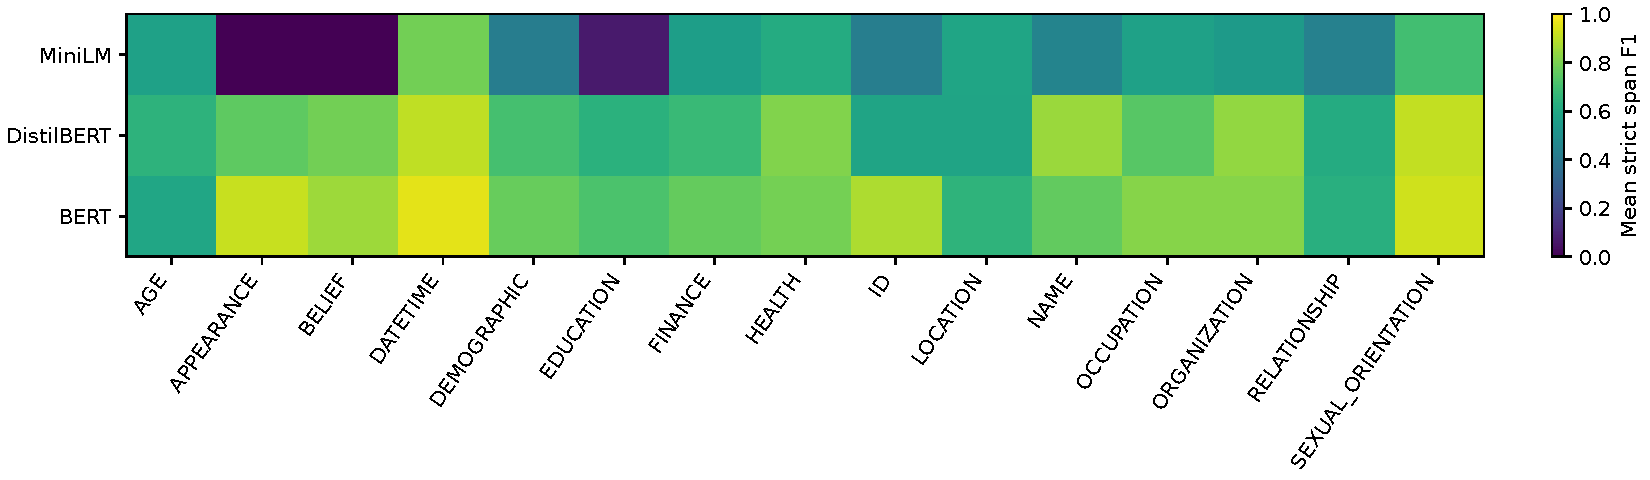
\includegraphics[width=\columnwidth]{../../figures/capid_per_type_f1.pdf}
\caption{Strict typed CAPID span F1 by category on the frozen 64-document prefix. Error bars show sample SD across three seeds.}
\label{fig:types}
\end{figure}

Per-type results reveal weaknesses hidden by aggregate F1. MiniLM records zero mean exact F1 for APPEARANCE and BELIEF and only 0.074 for EDUCATION. Its mean F1 drops from 0.588 on short contexts to 0.348 on long contexts. DistilBERT remains near 0.72--0.76 across length buckets. BERT rises from 0.752 on short contexts to 0.811 on long contexts. Supports are small, so these patterns remain exploratory.

\subsection{Training Data and Computational Cost}
Doubling the requested AI4Privacy subset from 5K to 10K improves strict span F1 by 0.0179 for MiniLM, 0.0158 for DistilBERT, and 0.0167 for BERT. Training time approximately doubles. At 10K, DistilBERT is 0.0019 F1 below BERT, while median detector latency is 30.7 rather than 57.4 ms. MiniLM is fastest at 13.1 ms but remains 0.0196 F1 below BERT.

\begin{figure}[t]
\centering
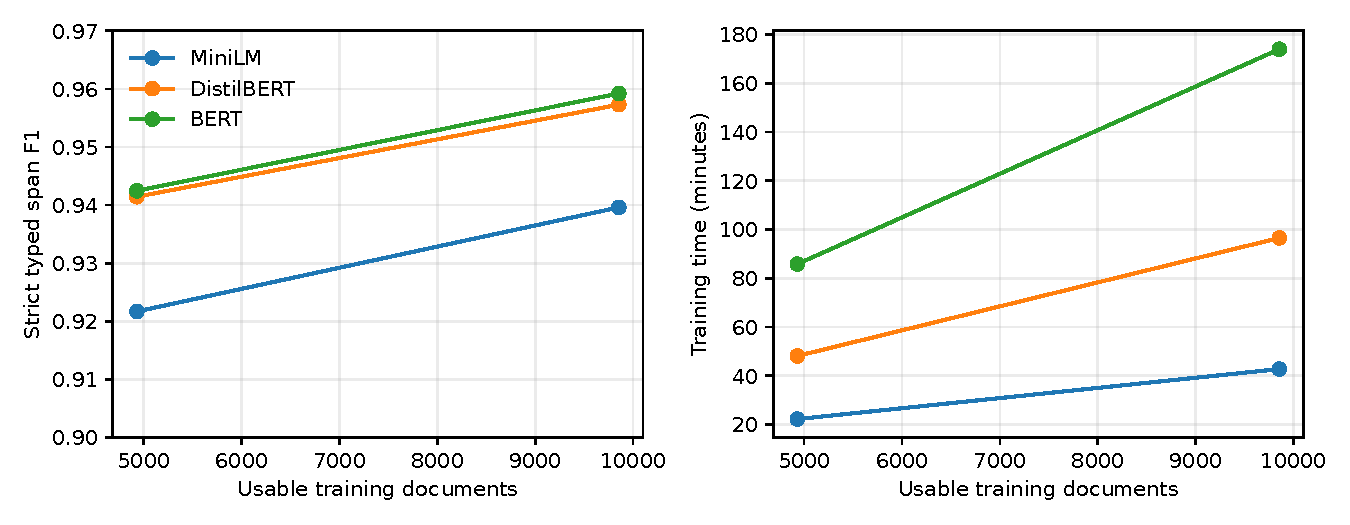
\includegraphics[width=\columnwidth]{../../figures/scaling_quality_cost.pdf}
\caption{Reduced seed-42 scaling study. More data improves every detector while training cost increases.}
\label{fig:scaling}
\end{figure}

Complete context-aware pipelines cost substantially more than detector-only inference because the relevance classifier runs once per detected entity. Median pipeline latency is 345 ms for MiniLM, 734 ms for DistilBERT, and 1,424 ms for BERT. Corresponding peak RSS is 585, 870, and 1,192 MiB.

\subsection{Privacy Trade-off and Domain Shift}
The 5\% primary target is infeasible for all nine model and seed pairs. Detector misses create a validation leakage floor above the target even under mask-all. At the frozen secondary point, BERT has the lowest mean retained-test leakage, 0.096, but also the lowest mean retention, 0.322. DistilBERT retains 0.478 with leakage 0.127. MiniLM leaks 0.183 while retaining 0.454.

\begin{figure}[t]
\centering
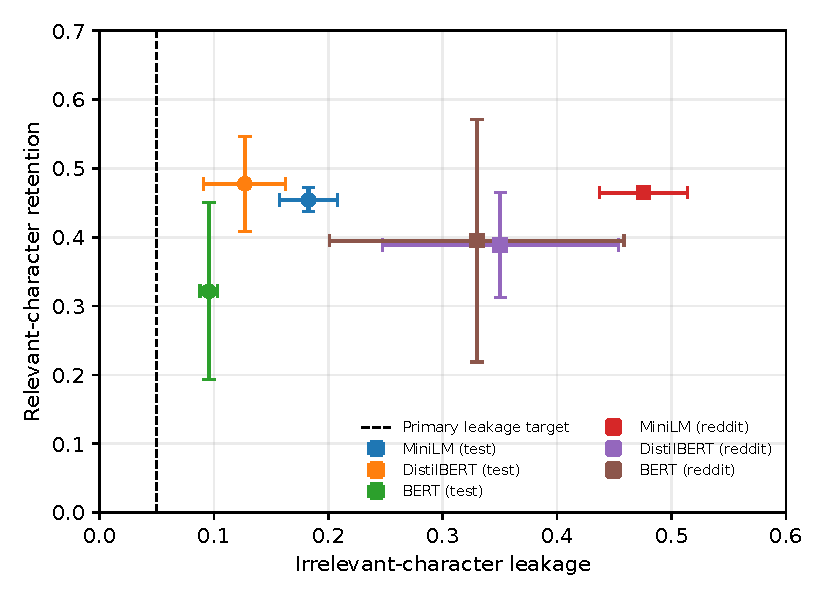
\includegraphics[width=\columnwidth]{../../figures/privacy_tradeoff.pdf}
\caption{Validation-locked floor-plus-five-percentage-point diagnostic. The dashed line marks the infeasible primary target.}
\label{fig:privacy}
\end{figure}

Reddit evaluation exposes a large domain shift. Mean leakage rises to 0.475 for MiniLM, 0.350 for DistilBERT, and 0.330 for BERT. This degradation may reflect writing style, category distribution, or both. The experiment does not isolate those causes.

\subsection{Qualitative Demonstration}
The local interface accepts a context, a task question, a model, and a policy. It shows detected spans, types, relevance scores, masking decisions, protected text, inference time, and current server RSS. Four short examples were checked across all three detectors. The recommended presentation setting uses BERT with mask-all because BERT produces the cleanest boundaries and types.

For the identity example, BERT converts ``My passport number is A1234567. I was born on 14 March 1998.'' into ``My passport number is [REDACTED]. I was born on [REDACTED].'' This example demonstrates the path, not general accuracy. Aggregate held-out results and failure cases remain the basis for conclusions.

\section{Discussion}
\subsection{Answer to RQ1}
No tested model satisfies every declared deployment criterion. MiniLM has the lowest latency and memory use, but its CAPID detector is substantially weaker and its question ablation shows almost no mean dependence. BERT detects best, but it has the highest latency and memory use, and one relevance seed collapses. DistilBERT gives the strongest measured compromise. It approaches BERT in the 10K detector study, leads mean relevance macro-F1, and requires less pipeline time and memory than BERT. This finding supports a practical choice, not a claim that DistilBERT meets the failed leakage requirement.

\subsection{Answer to RQ2}
Every model improves when usable AI4Privacy training data increases from 4,930 to 9,854 documents. Absolute F1 gains cluster between 0.016 and 0.018, while training time roughly doubles. The study cannot separate the value of additional unique documents from the larger number of optimizer steps because epochs remain fixed. A matched-update experiment would be needed for that causal distinction.

\subsection{Operational Implications}
Mask-all remains the appropriate default when disclosure cost is high. Context-aware retention should require validation on the intended domain, a documented leakage budget, and user-visible review. Current server RSS in the demonstration helps explain actual local footprint, while the paper retains controlled peak RSS for model comparison. The two measurements answer different questions and should not be mixed.

The examples also show why polished demonstrations must not replace error analysis. Some detectors split one real entity into several spans or assign the wrong type while still masking the full sensitive string. Other cases produce unwanted redaction in ordinary task text. A usable system needs stronger calibration, structured post-processing, and evaluation on natural user prompts.

\section{Reproducibility and Ethics}
The repository pins dataset and model revisions, records SHA-256 checksums, archives licenses, preserves raw sources, and writes every preprocessing exclusion. Run metadata includes configuration, code hash, parameter count, environment, elapsed time, and memory. Results remain machine-readable, and published reference values occupy a separate table from reproduced measurements.

The system processes examples locally and does not log prompt bodies. The demonstration uses synthetic identities. Users should not enter real confidential data during evaluation because missed PII can remain. Relevance does not imply consent, legal permission, or a need to transmit an identifier.

The reproducible path begins with checksum validation, rebuilds the derived summaries and figures from saved predictions, regenerates manuscript tables, and compiles the paper twice. Completed run directories remain immutable. New experiments require new identifiers, so a failed or altered run cannot silently replace an earlier result. Tests cover span alignment, leakage calculations, grouped splits, threshold selection, paired populations, and the local interface.

\balance
\section{Validity Considerations}
Internal validity depends on a common pipeline and deterministic settings, but model-specific optimization was intentionally limited. One learning rate and a small search space improve comparability while potentially disadvantaging a backbone. The relevance repair uses the same class-weighting rule for every model and derives weights from training labels only.

Construct validity is limited by the metrics. Exact typed spans penalize a nearly correct boundary and a wrong type equally, while character leakage gives partial credit to partial spans. Gold-span relevance isolates the classifier from detector errors, whereas full-pipeline leakage combines both components. Reporting the measures together prevents one score from standing in for the complete privacy problem.

External validity remains the largest concern. AI4Privacy is synthetic, CAPID pilots are small, and Reddit produces much higher leakage. The selected examples confirm that the software path runs as intended; they cannot estimate population performance. Conclusion validity is also limited for the one-seed scaling study. Its measured gains are descriptive rather than statistical evidence that one architecture benefits more from additional data.

\section{Limitations}
The multiseed experiments use small pilot subsets. The larger scaling study covers one seed and two data sizes. We did not run the planned 25K, full-data, matched-update, or GPU matrix. CAPID normalization excludes 114 training, nine test, and 28 Reddit records, mainly because flat BIO labels cannot represent overlapping spans. The retained population differs from the published CAPID protocol.

AI4Privacy is synthetic. Lexical duplicate audits do not establish semantic independence or real-world generalization. Entity-centered relevance crops may omit distant evidence. Character retention is not downstream question-answering utility. Process memory depends on runtime overhead, and laptop timing depends on background load. PII-Bench dataset access was not verified, so the project reports no reproduced PII-Bench result. No formal privacy guarantee, consent decision, or regulatory compliance claim is made.

\section{Conclusion}
EdgePII demonstrates a reproducible local pipeline for PII detection, contextual relevance estimation, and deterministic masking. More AI4Privacy data improves every detector in the reduced study. MiniLM minimizes cost but performs poorly after CAPID adaptation. BERT detects best at the highest resource cost and shows unstable relevance training. DistilBERT provides the most defensible accuracy and efficiency balance among the tested models. The primary leakage target nevertheless fails for every model because missed detections remain visible. Future work should prioritize recall, robust relevance training, natural-domain evaluation, and matched-compute scaling before adding optional compression methods.

\begin{thebibliography}{9}
\bibitem{capid} M. Ponomarenko, S. Abedini, M. Shafieinejad, D. B. Emerson, S. Mohapatra, and X. He, ``CAPID: Context-Aware PII Detection for Question-Answering Systems,'' arXiv:2602.10074, 2026.
\bibitem{piibench} H. Shen, Z. Gu, H. Hong, and W. Han, ``PII-Bench: Evaluating Query-Aware Privacy Protection Systems,'' arXiv:2502.18545, 2025.
\bibitem{ai4privacy} AI4Privacy, ``PII Masking 200K,'' Hugging Face dataset, \emph{ai4privacy/pii-masking-200k}, pinned revision, 2022.
\bibitem{bertpaper} J. Devlin, M.-W. Chang, K. Lee, and K. Toutanova, ``BERT: Pre-training of Deep Bidirectional Transformers for Language Understanding,'' in \emph{Proc. NAACL-HLT}, 2019.
\bibitem{distilbertpaper} V. Sanh, L. Debut, J. Chaumond, and T. Wolf, ``DistilBERT, a Distilled Version of BERT: Smaller, Faster, Cheaper and Lighter,'' arXiv:1910.01108, 2019.
\bibitem{minilmpaper} W. Wang, F. Wei, L. Dong, H. Bao, N. Yang, and M. Zhou, ``MiniLM: Deep Self-Attention Distillation for Task-Agnostic Compression of Pre-Trained Transformers,'' in \emph{Proc. NeurIPS}, 2020.
\bibitem{minilm} N. Reimers, ``MiniLM-L6-H384-uncased,'' Hugging Face model card, \emph{nreimers/MiniLM-L6-H384-uncased}.
\end{thebibliography}
\end{document}
